\section{Extended State of the Art}\label{sec:eSOTA}

\begin{displayquote}
\textit{\textbf{\Huge{``}}}
\textit{\large{
Kubernetes has massive potential for handling IoT workloads on the edge by providing a common control plane across hybrid cloud and edge environments to simplify management and operations\cite{ioFogMainBlog:online}.
}}
\textit{\textbf{\Huge{''}}}
\\[1pt]
\raggedleft{{\rm --- Mike Milinkovich, CEO of Eclipse Foundation}}
\end{displayquote}

\comment{
https://www.iaria.org/conferences2016/filesICSNC16/Softnet2016_Tutorial_Fog-MEC-Cloudlets-E.Borcoci-v1.1.pdf

this paper has it nailed down with terms https://arxiv.org/pdf/1812.00591.pdf 
}

\subsection{Terms and Definitions} \label{sec:definitions}
The IoT and edge landscape is hard to understand, especially because terms are loosely and inconsistently defined. Similar is true for the cloud but it uses less diverse technologies and is thus less confusing. This section will explain the network topology, key terms and their concepts as the foundation for the following report.\\
\vspace{0.5mm} \ \\
\textbf{\textit{Network Topology}}\\
\Cref{fig:networkTopology3Layer} shows the network topology used in this report. 
% The focus will be on the management and security of the device edge as well as its interaction with the IoT devices themselves. 
\begin{figure}[H]
    \centering
    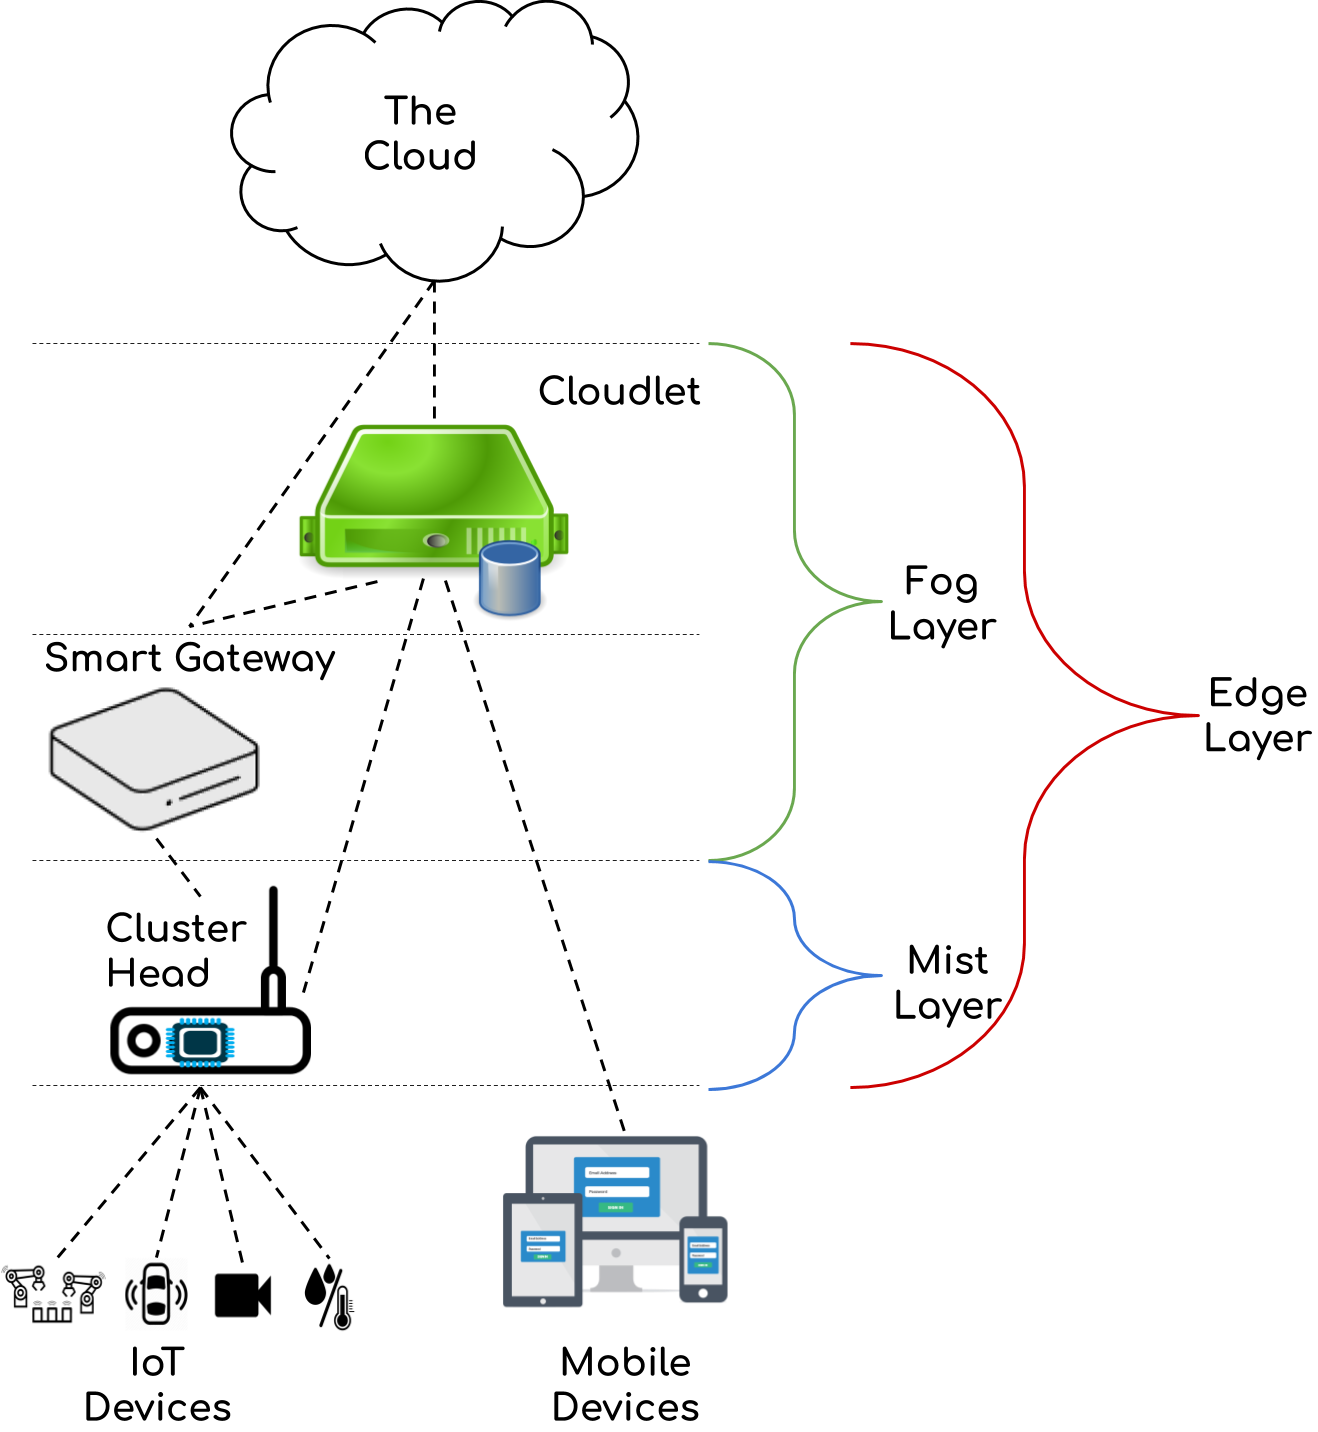
\includegraphics[scale=0.2]{figures/network-topology-3-layer.png}
    \caption{Three tier layer network topology, similar to \cite{nsa2017NextWaveIoTDef}}
    \label{fig:networkTopology3Layer}
\end{figure}

The cloud is well defined and understood. It describes the readily available computing resources over the Internet not managed by the user. The other layers and devices are not so well understood and defined separately.
\textbf{\textit{Constrained Device}}\\
Constraint devices are an elementary part of the IoT making up the "things"\cite{contstraintDevicesTerminology}.
They can have three main purposes. Either sensing or actuating (or both), where sensing is the 
passive action of measuring the environment (e.g. a motion detector) and actuating is the active action of influencing the environment (e.g. control of pressure in test tube). Or, finally, they can be smart objects enhancing the interaction between other smart objects and people.
They are usually defined by their limitation, mainly, small computing power (CPU, RAM, storage etc.) and limited power supply and operate in constrained network using protocols like BLE and ZigBee. \\[5mm]
\textbf{\textit{Smart/mobile devices}}\\
Smart devices are not clearly defined in the academic literature. I will use the definition given by \citeauthor{poslad2011smartDevices}\cite{poslad2011smartDevices}, to clearly divide them from constrained devices which this thesis will be concerned with. They are traditional computing devices and "tend to be multi purpose ICT devices"\cite{poslad2011smartDevices}, examples are mobile phones (smart phones) or tablets. They connect to the rest of the infrastructure directly but are free to move between networks. They also often rely on battery power and, importantly, are mainly end user devices. This has important privacy implication, a major factor for edge computing.\\[5mm]
\textbf{\textit{IoT Cluster Head}}\\
IoT Cluster Heads are defined by their very limited processing power. They are used to combine multiple sensors or actuators, but do not perform powerful operations. The line between IoT Cluster Heads and IoT Gateways is constantly moving as devices get more powerful and software more efficient. In this paper, IoT Cluster Heads are defined as devices which are used to read and control IoT devices but are not powerful enough to run containers or Kubernetes.
\textbf{\textit{IoT Gateway}}\\
IoT gateways are the connection between constrained devices and the cloud. I will use the term IoT gateway and not only gateway to stress its relation with IoT. They are usually connected to a network, either local or the the Internet. They facilitate inter-network and intra-network communications and because smart devices and especially constrained devices often communicate via wireless and non-Internet protocols, IoT gateways often translate protocols "between wireless sensor networks [...] and traditional communication networks"\cite{zhu2010iotGatewayDefinition}.
In recent years IoT Gateways have become a major field of interest and new research. As these devices got more powerful, developers started using them for pre-processing and data gathering locally at the edge.
IoT gateways can take a wide variety of forms. They can be simple L2/L3 routers or more powerful devices. Importantly, they are situated at the edge of a network.\\[5mm]
\textbf{\textit{Edge Layer}}\\
The edge layer is a term used to describe all resources sitting at the edge of the network. They do not interact with their environment directly only through IoT or mobile devices. This line started to fade, when mobile devices where used to control IoT devices directly. In this research I will stick to definition that edge layer devices are no user facing devices.\\[5mm]
\textbf{\textit{Fog Layer}}\\
The fog layer and consequently fog computing is a term used to describe the logical extension of traditionally cloud resources to the edge. These devices are still connected to the overall system and are an active part in the data processing pipeline. Fog computing enables repeatable structure on the edge for better and more scalable performance.
\textbf{\textit{Mist Layer}}\\
The mist layer is not logically connected to the cloud and both are not part of the same system and function independently of each other. It can be that the cloud can indirectly control the mist layer through the fog devices but importantly the mist layer does not do tasks which were traditional done in the cloud. \\[5mm]
\textbf{\textit{Edge cluster}}\\
Edge clusters are two or more edge devices working together where one device needs to be powerful enough to run a full control plane of the cluster technology. With emerging technologies like tiny builds of a full Kubernetes cluster, e.g. K3s from Rancher Labs\cite{k3sLight14:online}, this is becoming increasingly easier and more popular.
\footnote{Rancher provides a 40MB Kubernetes binary and claims that 500MB of RAM is sufficient 
it stable.}.\\
\textbf{\textit{Edge node}}\\
Edge nodes are defined as nodes "that act as an end user portal for communication with other
nodes in cluster computing"\cite{Whatised17:edgeNodeDef}. The other nodes can either be edge nodes as well or cloud nodes. Importantly, edge nodes do not need to be able to run their own control plane.
\subsection{Candidate Technologies}
<<<<<<< HEAD
Traditionally, edge devices were isolated gateways mainly forwarding traffic from their slaves to the cloud. This meant, all processing and storing was done in the cloud. Thus, the software of the gateways didn't need much management or maintenance. With advent of increased processing and storage at the edge, so called fog computing, the software on the gateways expanded to include business logic as well as routing. Today, gateways can be an integral part of the data flow, pre-processing data, filtering and storing data. However, this new software needs much more maintenance and management because changes in the business logic, e.g. API changes, need to be implemented in the gateway as well as on all other connected devices. With the advent of IIoT, the number of IoT gateways is set to increase dramatically and thus a solution for this problem has to be found.\\ This chapter will compare three different solutions for IoT gateways: Traditional gateway solutions, smart gateway solutions and gateways running on Kubernetes. First, a short overview of traditional gateway solutions is provided. Then, smart gateway solutions are defined and the Bosch IoT suite based on the OSGi technology is analyzed. Finally, gateway solutions based on kubernetes are presented and analyzed. The destinction between smart gateways and kubernetes based gateways is purely driven by kubernetes. It is the de-facto standard for cloud orchestration, has the support of (almost) all big IT companies and has many advantages over not so highly orchestration technologies.



The academic literature is not yet uniform in how to categorize IoT technolog

Open field --> work in progress so categories are not one implementation fits it all.

How should security be implemented.
Look into container and kubernetes security for IoT

How to solve low processing power of esp32?


provide many of the features cloud native (with containerization) do. Orchestrated solutions on the other hand offer a central configuration point, so a shared control plane between multiple gateways. These solutions were specifically developed for a distributed and large scale IoT environemnt. In many ways they are comparable to the solutions described in the next two subchapters, but are not developed with containerization at its foundation.

=======
Traditionally, edge devices were isolated cluster heads mainly forwarding traffic from their slaves to the cloud. Today, they are an integral part of the data flow pre-processing data and executing part of the business logic. But, there are still no coherent architectural as well as technological standards. In this section we will compare widely adopted and developed solutions in the industry to detect similarities and differences. The solutions also differ in age and 
>>>>>>> origin/overleaf-2019-07-23-0728
% https://scholar.google.com/scholar?cluster=13680069378267225814&hl=de&as_sdt=0,5
https://www.pac-online.com/sites/pac-online.com/files/upload_path/PDFs/Thema_des_Monats_Juni_2017_IoT_Plattformen.pdf
https://blog.bosch-si.com/bosch-iot-suite/lessons-learned-using-kubernetes-in-iot-deployments/

\subsection{Categorization of Gateways.}

<<<<<<< HEAD

\subsection{Traditional Gateway Solutions}
Tradition gateway solutions are all solutions which do not interact with data or only in a very limitted way and usually not content based. They are thus mainly forwarding data, i.e. operating as L3 device. The software running these devices is usually pre-installed by an OEM and hard to update and maintain. The gateways are isolated and information is only accumulated and processed in the cloud. Multiple gateways do not have a shared or centralized control plane and thus need to be managed independently and locally.\\
As these devices are still widely popular, they will form the base or reference case for this analysis. Compared to the next solutions, technologies in this category are not considered to do fog computing.


\subsection{Smart Gateway Solutions}
https://www.bosch-iot-suite.com/service/gateway-software/
Smart gateway solutions are all solutions which interact with their data on a business level perspective.

Smart gateway def  quotes:

[13] Internet of Things with Cloud Computing and the Issues Involved”, in
the proceedings of 11th IEEE International Bhurban Conference on
Applied Sciences and Technology, Islamabad, Pakistan, 14-18 January,
2014.
[14] Mohammad Aazam, Eui-Nam Huh, “Smart Gateway Based
Communication for Cloud of Things”, in the proceedings of 9th IEEE
International Conference on Intelligent Sensors, Sensor Networks, and
Information Processing, Singapore, 21-24 April, 2014.


But, they do not employ any cloud technologies like containers or kubernetes, even though the design philosophies are often overlapping. They may have a fully centralized configuration and control plane offering a central configuration point for multiple gateways or only parts of it. They may also take advantage of isolation to abstract in some form the underlying hardware.\\
The OSGi technology\cite{osgiDefintion25:online} is a aliance driven project from the Open Services Gateway initiative. It is a set of specifications (with reference implemetation and tests) for a dynamic modular system based on so called bundles, third party software, running on the Java Virtual Machine (JVM)\footnote{This means it is possible to use other languages apart from Java which can run in a JVM, e.g. Kotlin or Scala.}. The solution consists of a layered model shown in \cref{fig:osgiLayerModel}. 
=======
\subsubsection{Bosch IoT Gateway Solutions}
\comment{https://www.bosch-iot-suite.com/service/gateway-software/}
The Bosch IoT Gateway Software\cite{BoschIoT13:online} is the "oldest" software analyzed. It is based on the OSGi technology\cite{osgiDefintion25:online}, which is an aliance driven project from the Open Services Gateway initiative (OSGi). It defines a set of specifications (with reference implemetation and tests) for a dynamic modular system based on so called bundles, third party software, running on the Java Virtual Machine (JVM)\footnote{This means it is possible to use other languages apart from Java which can run in a JVM, e.g. Kotlin.}. It is important to note that Bosch also supplies a cloud part which is based on Kubernetes.\\
The OSGi framework consists of a layered model shown in \cref{fig:osgiLayerModel}. 
>>>>>>> origin/overleaf-2019-07-23-0728
\begin{figure}[h!]
    \centering
    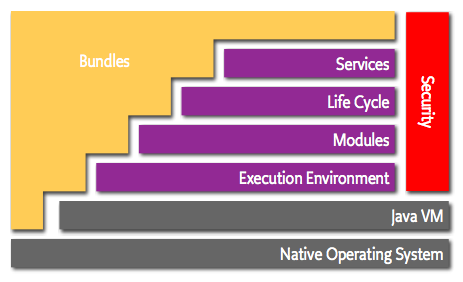
\includegraphics[scale=0.8]{figures/layering-osgi.png}
    \caption{From the official OSGI documentation\cite{osgiFrameworkArchitec22:online}.}
    \label{fig:osgiLayerModel}
\end{figure}
<<<<<<< HEAD
The Service layer interconnects the bundles making it possible for them to communicate via plain old java objects (POJO).The Life-Cycle layer handles the the state of the application (start, stop, update and uninstall). The Modules layer defines how an application can import and export code and the Execution Environemnt defines which methods and classes are available in a specific environemnt. Finally, the Security layer encompases all other layers and handles for example code authentication, the digital signing of jar files, file access restrictions, certificates and more.\\
There are currently six frameworks implementing the OSGi model which are under active development\footnote{This is to the authors best knowledge. Active development means, that security updates are still provided.}. One such solution is the Bosch IoT Gateway Software\cite{BoschIoT13:online}. In a blog entry from 2015 Bosch compares the OSGi technology to other gateway solutions and says it "is the only one with clearly defined specs and an open specification process behind them"\cite{boschBlogOSGi69:online}. Boschs solution is proprietary and tailer made for edge-computing devices with IIoT in mind\cite{OSGiforIoTBlog27:online}. It runs on Linux, Windows, mac OS, Android, and VxWorks and according to Bosch more than 40 different gateway devices\cite{BoschIoT13:online}. The software is stable at major version 9 and still under heavy development. Because of these reasons, it is used as an examplary solution. \Cref{fig:boschIoTGatewaySetup} shows where Boschs IoT solution is situated in the IoT environment. Bosch provides the OSGi framework implementation for the gateways and additional features for the cloud to ease the management of the gateways and store the accumulated data.
=======
The Service layer interconnects the bundles making it possible for them to communicate via plain old java objects (POJO).The Life-Cycle layer handles the the state of the application (start, stop, update and uninstall). The Modules layer defines how an application can import and export code and the Execution Environemnt defines which methods and classes are available in a specific environemnt. Finally, the Security layer encompasses all other layers and handles for example code authentication, the digital signing of jar files, file access restrictions, certificates and more.\\
To the authors best knowledge there are currently five frameworks implementing the OSGi model besides the Bosch IoT Gateway Software\cite{BoschIoT13:online}. In a blog entry from 2015 Bosch compares the OSGi technology to other gateway solutions and says it "is the only one with clearly defined specs and an open specification process behind them"\cite{boschBlogOSGi69:online}. Boschs solution is proprietary and tailor made for edge-computing devices with IIoT in mind\cite{OSGiforIoTBlog27:online}. It runs on Linux, Windows, mac OS, Android, and VxWorks and according to Bosch more than 40 different gateway devices\cite{BoschIoT13:online}. The software is stable at major version 9 and still under heavy development. It is presented as exemplary software by the OSGi Alliance for IoT Gateways \cite{exampleIoTGateweOSGi:online} and thus used in this report. \Cref{fig:boschIoTGatewaySetup} shows where Boschs IoT solution is situated in the IoT environment. Bosch provides the OSGi framework implementation for the gateways and additional features for the cloud to ease the management of the gateways and store the accumulated data.
>>>>>>> origin/overleaf-2019-07-23-0728
\begin{figure}[h!]
    \centering
    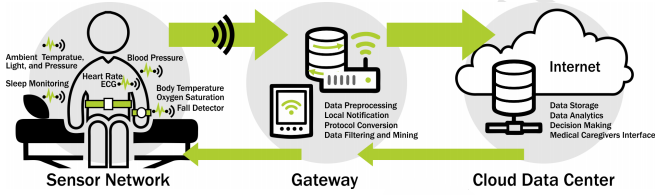
\includegraphics[scale=0.8]{figures/iotSetup.png}
    \caption{From the official Bosch documentation \cite{BoschIoT13:online}.}
    \label{fig:boschIoTGatewaySetup}
\end{figure}
Moreover, it supports a wide variety of communication protocls, BLE, ZigBee and MQTT, just to name a few. The main restriction is the JVM support for a protocol.  

\subsubsection{ioFog}
ioFog is one of the older projects in this report, with the first official release in 2016\cite{ioFogMainBlog:online}. Similarly to the OSGi framework it provides a runtime environment for applications, mainly intended for microservices. In addition, it includes a message bus, dynamic configuration of the microservices, and remote debugging\cite{ioFogMainBlog:online}. It runs on (almost) all Linux distributions and only requires Docker to be installed. In their official system requirements they only recommed using a Raspberry Pi as a worker node and not to run the Controller and Connector infrastructure \cite{ioFOgQuickStart:online}.
\Cref{fig:ioFogComponent} shows the fog computing layers in more detail.
\begin{figure}[h!]
    \centering
    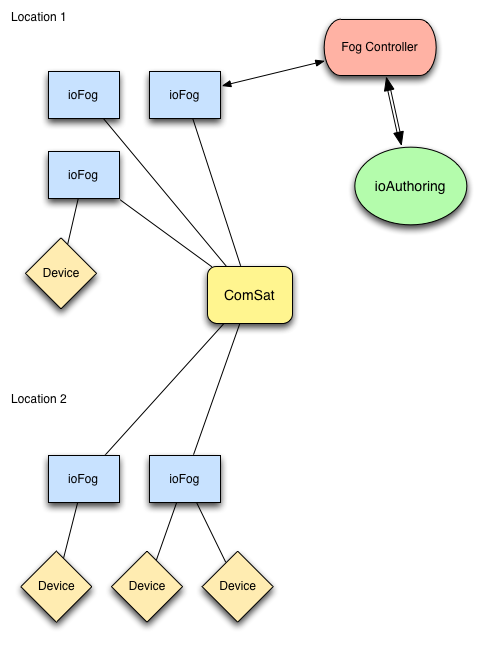
\includegraphics[scale=0.4]{figures/ioFog-Component_Diagram.png}
    \caption{hallo}
    \label{fig:ioFogComponent}
\end{figure}\\
The ioAuthoring application and the ioFog instances provide orchestration and management of the microservices. They are the main interaction points between the administrator and the system.
The fog computing software agent, called "ioFog", runs on various operating systems and provides a universal runtime for the IoT microservices. It includes a Software Development Kits (SDKs) in multiple programming languages to provide developers with the convenience of programming against standardized objects. The communication between different ioFog instances is facilitated through an internetworking utility that runs on popular Linux distributions, called "ComSat". Finally, for testing a tool for mimicking the fog computing runtime is included as well.\\
In a recent blog post from Mike Milinkovich, the Executive Director of the Eclipse Foundation Inc., he announced the initial availability of ioFog features that make any Kubernetes distribution edge-aware. He continuous saying that "these native Kubernetes enhancements are in the process of being contributed to the Eclipse ioFog open source project.", so not all features are available in the stable release as of the time of writing. But essentially, the ioFog Kubernetes APIs would provide standardized way of communication between the Kubernetes API Server and the ioFog instance.

\subsubsection{Docker Edge Solution}
Docker is commonly known for its containerization software and is often confused with the containers themselves (like google for search). The core container runtime, containerd, was donated by Docker to the Cloud Native Computing Foundry (CNCF) in 2017\cite{containerDonationDocker79:online} which manages and develops it now. Now, the company Docker focuses on providing an ecosystem around containers making them easy to deploy, secure and replicate. Recently, Docker announced a new partnerships with ARM and  a new strategy for edge devices.\\
\Cref{fig:dockerEdge} shows the Docker Edge Solution in context. 
\begin{figure}[h!]
    \centering
    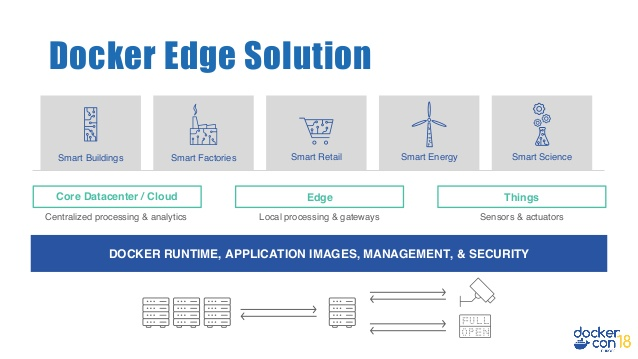
\includegraphics[scale=0.65]{figures/docker-edge-solution.jpg}
    \caption{Docker Edge solution .}
    \label{fig:dockerEdge}
\end{figure}
The solution consists of a few different products from its enterprise solution focusing on security, scalability/deployability and easy of use. The components are the same, but the edge focus is on fault tolerance and platform support, hence the new partnership with ARM. A core component of the suit is the docker registry, which can be mirrored/replicated on many difference servers for scaleability and fault tolerance. The edge registry can function without constant communication with the rest of the swarm. In case of no connection, the registry will only pull images which it already posses. As edge devices often have limitted disk space, docker only synchronizes promoted images on these nodes. Similarly to tags in git, promoted images are signed images that are explicitly marked as production ready. \cref{fig:dockerRegistryForIoT} shows registry management in the cloud (on the left) vs. on the edge (on the right).
\begin{figure}[h!]
    \centering
    \noindent\makebox[\textwidth]{
    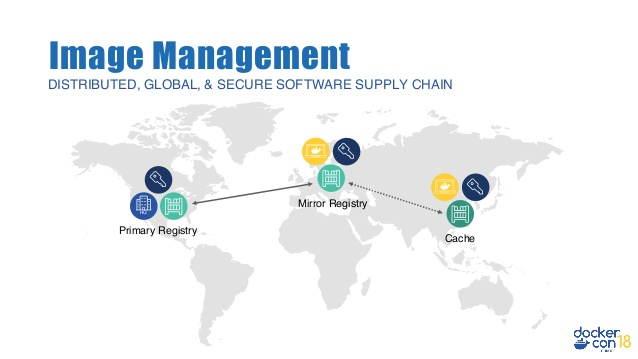
\includegraphics[width=(\textwidth+4cm)/2]{figures/docker-edge-computing-with-docker-enterprise.jpg}
    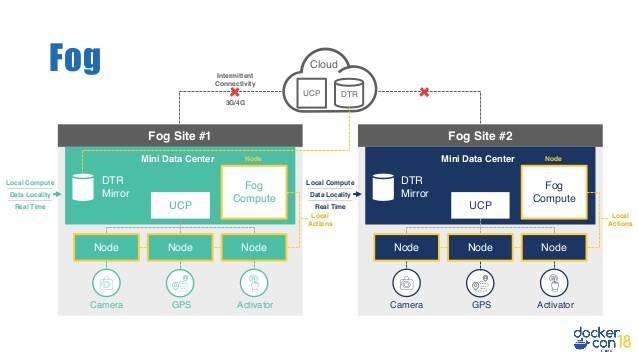
\includegraphics[width=(\textwidth+4cm)/2]{figures/docker-edge-registry-mirror.jpg}}
    \caption{The Docker registry in the cloud (left) vs. on the edge (right).}
    \label{fig:dockerRegistryForIoT}
\end{figure}
Whereas the cloud registry is build high availability (HA/LB) of the nodes in the swarm with fault tolerance against other nodes being unavailable, the edge registry is designed to have fault tolerance on it's own Internet access. In case of no connection it works as a standalone component, but synchronizes itself when it has a connection.\\
Importantly, the Docker Edge Solution is not a standalone solution, but integrates into the Docker ecosystem enabling remote management.

\subsubsection{K3s}
K3s is a "lightweight" kubernetes\footnote{Kubernetes is also known as k8s, hence the name k3s.} fork developed by Rancher\cite{rancherMainPage:online}. Similarly to Kubernetes and containerd, k3s is an open source project under the official management of the CNCF. It is also part of the Kubernetes IoT Edge working group explicitly aiming at bringing kubernetes related technologies to the edge. K3s is also a Certified Kubernetes distribution, meaning it confirms with the Kubernetes API standards. One of its big selling points is the good support for ARM64 and ARMv7 (targeting the Raspberry Pi and other smaller/less powerful single board computers). The traditional Kubernetes development is focused around the x86\_64 architecture, with limitted, and often untested, support for ARM, especially ARMv7. The co-founders of Rancher and developers behind k3s actually state in a webinar that half their development effort went into ensuring that all features they wanted work seamlessly on ARM\cite{k3sTalk:online}.\\
On their k3s product page \url{https://k3s.io/} Rancher describes the fork as follows:
\begin{displayquote}
Easy to install. A binary of less than 40 MB. Only 512 MB of RAM required to run.
\end{displayquote}
So k3s is not only significantly smaller than the full fledged Kubernetes install, but also requires significantly less resources at run time. It achieves this by mainly slimming down Kubernetes only including what they deem important for the edge. Because of the huge popularity of Kubernetes, it needs to support legacy code, drivers etc. K3s is free to break compatibility with older versions and the developers can instead focus on slimming down the code base much as possible. The lead developer, Darren Shepherd, said:
\begin{displayquote}
\textit{"We took Kubernetes and ripped out every single feature we didn't want.\cite{k3sTalk:online}"}
\\[1pt]
\raggedleft{{\rm --- Darren Shepherd}}
\end{displayquote}
K3s also integrates all process required by Kubernete, the Kubernetes master, Kubelet and containerd under one system process which requires less memory in total. \\
Another important aspect of k3s is its purpose to run on single as well as multi-node clusters. This is in stark contrast to Kubernetes, which is intended to run inside a cluster and it's fault tolerance model is build around on a multi-node cluster structure. Running a single node cluster is possible, but requires the tainting of the master node and is describe as "cheap and easy, but is not production grade" in the official documentation\cite{singleNodeKubernetesNotProductionDocumenhtation:online}.

\subsubsection{Kubeedge}
Kubeedge is another project inside the Kubernetes IoT Edge working group and thus build with Kubernetes in mind. It is a relatively young project to extend native containerized application orchestration and device management to the Edge. It is based on two parts, the cloud and the edge and (mainly) developed by Huawei, which at the time of writing could be reason for future complications because of recent US sanctions against the company.\\
The kubeedge system is shown in \cref{fig:kubeedgeStruct}.
\begin{figure}[h!]
    \centering
    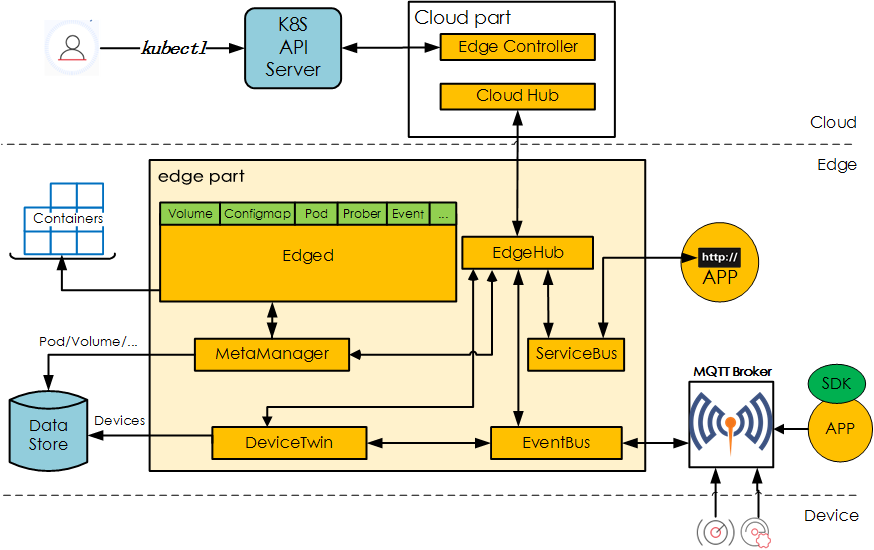
\includegraphics[width=(\textwidth+4cm)/2]{figures/kubeedge_arch.png}
    \caption{The Kubeedge system design.}
    \label{fig:kubeedgeStruct}
\end{figure}
The cloud part is built upon Kubernetes and provides support for application deployment, metadata synchronization and networking all through the Kubernetes API Server. The cloud and edge part communicate via web sockets. This means by design a good connection to the server is expected and the intend of the authors is to enable Fog computing. It is built upon Kubernetes and provides core infrastructure support for networking, application deployment and metadata synchronization between cloud and edge.\\
The edge part is not based on Kubernetes but uses similar concepts: Pods, volumes, events and more. It provides a life cycle management for containers and supports MQTT for communication for additional components. It also stores and synchronizes the device status to the cloud and has a query interface for local applications.


<<<<<<< HEAD
\subsection{Containerized Gateway Solutions}

IoT cluster solutions\\
Isolated k8s cluster: Solution k3s\\
Kubernetes cluster where edge is part of the cloud: kubeedge\\
% https://github.com/kubernetes/website/pull/13158



\subsection{Cloud Native Gateway Solutions}
Edged: an agent that runs on edge nodes and manages containerized applications.
EdgeHub: a web socket client responsible for interacting with Cloud Service for the edge computing (like Edge Controller as in the KubeEdge Architecture). This includes syncing cloud-side resource updates to the edge, and reporting edge-side host and device status changes to the cloud.
CloudHub: a web socket server responsible for watching changes at the cloud side, caching and sending messages to EdgeHub.
EdgeController: an extended kubernetes controller which manages edge nodes and pods metadata so that the data can be targeted to a specific edge node.
EventBus: a MQTT client to interact with MQTT servers (mosquitto), offering publish and subscribe capabilities to other components.
ServiceBus: a HTTP client to interact with HTTP servers (REST), offering HTTP client capabilities to components of cloud to reach HTTP servers running at edge.
DeviceTwin: responsible for storing device status and syncing device status to the cloud. It also provides query interfaces for applications.
MetaManager: the message processor between edged and edgehub. It is also responsible for storing/retrieving metadata to/from a lightweight database (SQLite).

https://randomnerdtutorials.com/esp32-over-the-air-ota-programming/

file:///home/joe/Downloads/DDoS%20in%20the%20IoT%20Mirai%20and%20Other%20Botnets.pdf
Security containers:
Mirai attack: weak passwords, needs shell
Counter: Docker, binary files, non root user, 
traffic analysis via istio
=======
\subsubsection{Conclusion}
Only recently have industry behemoths like, Docker, Huawei, Bosch, Siemens, Red Hat, VMware and more\cite{K8sattheEdgeContectOnWorkingGroup:online} started to develop and, more importantly, concentrate their efforts on integrated IoT Gateway solutions. This lack of standardization is also acknowledged by the developers themselves ``While the problems at the IoT edge — connectivity, manageability, scalability, reliability, security — are being solved as point solutions by enterprises and ecosystem players, there is a need for a foundational industry-wide standard for managing distributed IoT workloads.''\cite{ioFogK8sBlog:online}\\
\Cref{tab:shortSotaSoftware} shows how the different solutions analyzed in this section compare to each other in key aspects.
% \footnote{An extended version can be found in the appendix.}
\begin{table}[h!]
% \hspace*{-2cm}
    \begin{center}
        
    \noindent\makebox[\textwidth]{
\resizebox{\columnwidth}{!}{%
\begin{tabular}{l|lll p{2.5cm} lllll}
                  & \begin{tabular}[c]{@{}l@{}}Open\\Source\end{tabular} & \begin{tabular}[c]{@{}l@{}}Centralized \\ control plane\end{tabular} & SW   &  Protocols  & \begin{tabular}[c]{@{}l@{}}System Req\\ control plane\end{tabular} & \begin{tabular}[c]{@{}l@{}}System Req\\ worker node\end{tabular} & \begin{tabular}[c]{@{}l@{}}Container\\based\end{tabular} & \begin{tabular}[c]{@{}l@{}}Kubernetes\\ in cloud\end{tabular} & \begin{tabular}[c]{@{}l@{}}Kubernetes\\ on edge\end{tabular} \\ \cline{1-10} 
Bosch IoT         & No                                                                                                                             & Yes (cloud)                                                                                                                                  & Java & ZigBee, Z-Wave, BLE and more        & Server grade                                                                                                                               & Edge grade                                                                                                                               & No                                                                                                                                & Some                                                                                                                                  & No                                                                                                                                   \\
ioFog             & Yes                                                                                                                            & Yes (cloud)                                                                                                                                  & Java & ZigBee, Z-Wave, BLE and more        & Server grade                                                                                                                               & Edge grade                                                                                                                               & Yes                                                                                                                               & Some                                                                                                                                  & No                                                                                                                                   \\
Docker\\Enterprise & No                                                                                                                             & Yes (cloud)                                                                                                                                  & Go   & ZigBee, Z-Wave, BLE and more        & Server grade                                                                                                                               & Edge grade                                                                                                                               & Yes                                                                                                                               & No                                                                                                                                    & No                                                                                                                                   \\
K3s               & Yes                                                                                                                            & Yes (both)                                                                                                                                   & Go   & Only IP based protocols             & Edge grade                                                                                                                                 & Edge grade                                                                                                                               & Yes                                                                                                                               & Yes                                                                                                                                   & Yes                                                                                                                                  \\
Kubeedge          & Yes                                                                                                                            & Yes (cloud)                                                                                                                                  & Go   & MQTT and IP. More planned & Server grade                                                                                                                               & Edge grade                                                                                                                               & Yes                                                                                                                               & Yes                                                                                                                                   & No                                                                                                                         
\end{tabular}}}
    \caption{Summary of the analyzed software.}
    \label{tab:shortSotaSoftware}
    \end{center}
\end{table}
It is important to bear in mind, that the Bosch IoT solution as well as ioFog are significantly older than the other projects. Boschs IoT solution is based on the OSGi framework. It provides isolation evolving around the JVM. This enables it to be platform independent, that is as long as the OS provides a JVM. ioFog which is almost three years old as of time of writing (June 2019) and already relays on containers, specifically a Docker runtime, for its deployment.\\
As the second last column shows all solutions, except for Docker Edge, use Kubernetes as their orchestration platform and control plane of choice. ioFog and Bosch IoT Edge are currently updating their solution while Kubeedge and K3s where designed from the ground up with Kubernetes in mind. However, only K3s tries to bring Kubernetes to the edge as well. This also means, that all solutions require different hardware requirements for the control plane, usually server grade hardware running containers, and more resource efficient solutions for the edge. \\
It is also important to note that all newer solutions, Docker Edge Solution\footnote{As the source code is not publicly available, this is speculative based on the fact that the main programming language for Docker is Go.} K3s and Kubeedge is Go. Older systems are mainly based on Java as it enables code to run on every platform supporting the JVM. It is also important to note, that containers give developers freedom of programming language. The Bosch IoT Edge Solution and its use of the OSGi framework force developers into using a JVM compatible programming language. Docker points out that its solution runs on MacOS and Windows, however, both rely on Linux system calls.\footnote{Docker on Windows uses the WSL 2.0 in the future which translates Linux system calls to Windows system calls and increases performance a lot compared to emulated solutions as done on MacOS.}.\\
Another important aspect is protocol support. Here, the OSGi framework is clearly ahead as it has complete access to the system hardware, due to the JVM and also 



% From a design perspective, this is very similar to containers, where isolation is provided by Cspaces and Namespaces instead of process ID. Containers need access to communication 

% Giving access to devices like  Blt sigbee is a security issue.
>>>>>>> origin/overleaf-2019-07-23-0728



\comment{
Should I include Azure IoT Edge as managed cloud iot gateway offering????\\

The problems at the IoT edge, connectivity, manageability, scalability, reliability, security, are being solved as point solutions by enterprises and ecosystem players, there is a need for a foundational industry-wide standard for managing distributed IoT workloads.


What is the purpose of this section?\\
problem area: what is actually the problem with the current system? hint into solution\\
competitor anaylsis: compare different approaches to solve the management and security of IoT gateways as well as solutions inside the individual categories. 


}